\documentclass[onecolumn]{IEEEtran}
\IEEEoverridecommandlockouts
\usepackage{tikz}
\usetikzlibrary{shapes, arrows, positioning}
\usepackage{float}
\usepackage{booktabs}
\usepackage[center]{caption}
\usepackage{xcolor}

\title{A multimodal evaluation model for improving pedagogical outcomes}

\author{
    \IEEEauthorblockN{Shafiqul Islam} \\
    \IEEEauthorblockA{
        \textit{Begum Rokeya University,Rangpur} \\
    }
}

% Add these to your preamble for figures and tables


\begin{document}

\maketitle

\begin{abstract}
Teacher performance evaluation is a cornerstone of educational quality assurance. Traditionally, student feedback has been the primary tool for assessing teaching effectiveness, but it is often subjective and limited in scope. This proposal outlines a comparative study between a novel multimodal system—which objectively analyzes classroom interactions—and conventional student feedback. The study aims to determine the reliability, validity, and impact of both approaches.
\end{abstract}

\begin{IEEEkeywords}
Teacher evaluation, multimodal system, student feedback, educational assessment, comparative study
\end{IEEEkeywords}

% This is now Chapter 1

The evaluation of teacher performance is a cornerstone of educational quality assurance and institutional improvement \cite{Heffernan2022}. Effective teaching not only enhances student learning outcomes but also shapes the reputation and development of educational institutions \cite{Ajmal2024}. Traditionally, the assessment of teaching effectiveness has relied heavily on student feedback, which, while valuable, is often subject to various biases and limitations \cite{Heffernan2022}. These include subjectivity, inconsistency, and the influence of non-academic factors such as personal rapport, grading leniency, or classroom environment \cite{Steinberg2021}. Research has shown that demographic factors, such as gender and race, can also influence student evaluations, raising concerns about fairness and validity \cite{Steinberg2021}.

Despite these drawbacks, student feedback remains prevalent due to its simplicity, cost-effectiveness, and ability to capture students' perspectives on teaching quality \cite{Ajmal2024}. However, the reliability of student feedback is challenged by inconsistencies across different cohorts and courses, as well as by the tendency for students to focus on surface-level attributes rather than deeper pedagogical competencies \cite{carvalho2022biases}. Several studies have highlighted the need for more robust and objective evaluation mechanisms to complement or replace traditional feedback \cite{Ginsburg2022NecessaryBI}.

Recent advancements in educational technology have paved the way for more objective and comprehensive evaluation methods \cite{Wang2022}. Among these, multimodal systems that leverage data from multiple sources—such as audio, video, gesture recognition, and classroom interaction analytics—offer promising alternatives \cite{10.1007/978-981-99-9109-9_7}. These systems can provide a holistic view of teacher performance by capturing a wide range of behavioral and communicative cues that are often overlooked in traditional feedback mechanisms.

Artificial intelligence (AI) and machine learning (ML) techniques have enabled the automated analysis of complex classroom behaviors, including teacher movement, speech patterns, engagement strategies, and student responses \cite{Wang2022}. For instance, pose estimation algorithms can detect and classify teaching activities, while emotion recognition systems can assess the affective climate of the classroom. These technologies not only enhance the objectivity of evaluations but also provide granular feedback that can inform targeted professional development \cite{YE2023108915}.

Despite the potential of multimodal systems, there is a lack of empirical studies comparing their effectiveness with conventional student feedback \cite{Ginsburg2022NecessaryBI}. This research aims to bridge this gap by conducting a comparative study between a multimodal teacher performance evaluation system and traditional student feedback methods. The primary objectives of this study are to:

\begin{itemize}
    \item Analyze the strengths and weaknesses of both evaluation approaches \cite{Heffernan2022, carvalho2022biases, 10.1007/978-981-99-9109-9_7}.
    \item Assess the reliability and validity of multimodal data in reflecting true teaching effectiveness \cite{Wang2022, Yang2022, YE2023108915}.
    \item Investigate the correlation between multimodal system verdicts and student perceptions \cite{Ajmal2024, Husain2016, falcon2024discourse}.
    \item Provide recommendations for integrating advanced evaluation systems into existing educational frameworks \cite{Ginsburg2022NecessaryBI, 10.1007/978-981-99-9109-9_7, hou2024encouragement}.
\end{itemize}

The remainder of this book is organized as follows: Chapter 2 reviews related work in teacher evaluation and multimodal systems. Chapter 3 describes the proposed methodology, including data collection and analysis techniques. Chapter 4 presents the experimental setup, including classroom environment, hardware, and dataset details. Chapter 5 details the multimodal system architecture and implementation, including the system pipeline (see Figure~\ref{fig:multimodal_architecture}) and output classification (see Table~\ref{tab:output_categories}). Chapter 6 presents the results and discussion, and Chapter 7 concludes with final remarks and future directions.

The integration of multimodal systems into teacher evaluation frameworks represents a significant shift in educational assessment paradigms. These systems not only address the limitations of traditional feedback but also align with broader trends in educational technology and data-driven decision-making. For instance, the use of machine learning algorithms to analyze multimodal data streams enables the identification of nuanced teaching behaviors that correlate with student engagement and learning outcomes. Furthermore, the adoption of such systems has practical implications for teacher training and professional development, as they provide actionable insights that can guide instructional improvement.

However, the implementation of multimodal evaluation systems is not without challenges. Issues such as data privacy, the need for robust validation across diverse educational contexts, and the potential for algorithmic bias must be carefully considered. Despite these challenges, the potential benefits of multimodal systems—such as enhanced reliability, validity, and comprehensiveness—make them a promising complement to traditional student feedback. This study aims to explore these dynamics by conducting a comparative analysis of both evaluation approaches, thereby contributing to the growing body of literature on innovative educational assessment methods.


% This is now Chapter 2

\subsection{Student Feedback-Based Evaluation}
Student feedback has long been the predominant method for evaluating teaching effectiveness in higher education. Its widespread use is attributed to its simplicity, cost-effectiveness, and ability to capture students' perspectives on instructional quality \cite{Ajmal2024, Husain2016}. However, research has consistently highlighted significant limitations, including subjectivity, bias, and the influence of non-academic factors such as instructor popularity, grading leniency, and course difficulty \cite{Heffernan2022, carvalho2022biases}. Demographic factors, such as gender and race, can also affect student evaluations, raising concerns about fairness and validity \cite{Steinberg2021}. These issues have prompted calls for more objective and reliable assessment methods \cite{Ginsburg2022NecessaryBI}.

Despite its limitations, student feedback remains a central component in most institutional evaluation frameworks. Many universities rely on end-of-term surveys or online platforms to collect student opinions, which are then used for faculty appraisal, promotion, and professional development \cite{8615171}. However, the overreliance on student feedback can sometimes lead to unintended consequences, such as grade inflation or a focus on entertainment over educational rigor. Furthermore, the lack of standardization in survey instruments and interpretation of results can introduce inconsistencies across departments and institutions. Recent studies have also explored the psychological impact of student evaluations on teachers, noting increased stress and potential discouragement among faculty who receive negative or biased feedback. These findings underscore the need for complementary evaluation methods that can provide a more balanced and holistic view of teaching effectiveness.

\subsection{Auditory-Based Evaluation}
Auditory-based evaluation methods analyze audio data from classroom interactions to assess teaching performance. Techniques in this domain include speech recognition, prosody analysis, and emotion detection from vocal cues. These approaches can provide insights into teacher-student engagement, clarity of instruction, and the emotional climate of the classroom. Machine learning and signal processing advancements have enabled more accurate and automated auditory assessments, though challenges remain in handling noisy environments and diverse speaking styles \cite{Wang2022, Yang2022}.

In the context of teacher evaluation, auditory analysis offers a unique perspective by focusing on the nuances of verbal communication. For example, the tone, pace, and modulation of a teacher's voice can influence student engagement and comprehension. Studies have shown that enthusiastic and expressive speech is often associated with higher student motivation and participation. Additionally, auditory features can be used to detect classroom dynamics, such as the frequency of teacher-student interactions or the presence of collaborative discussions. Integrating auditory data with other modalities can help address the limitations of purely subjective feedback, offering a more objective measure of classroom engagement and instructional quality.

\begin{figure}[t]
    \centering
    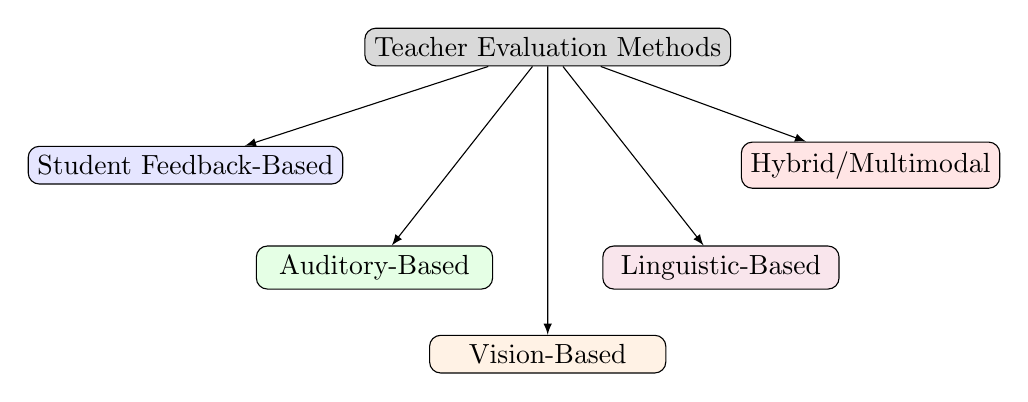
\begin{tikzpicture}[
        scale=2, % Adjusted scale for compactness
        level distance=0.8cm,
        sibling distance=1cm, % Further reduced for compactness
        every node/.style={font=\normalsize, align=center, draw, rectangle, rounded corners, minimum width=3cm, fill=gray!10},
        edge from parent/.style={draw, -latex}
    ]
    % Root node
    \node[fill=gray!30] {Teacher Evaluation Methods}
        child { node[fill=blue!10, yshift=0.1cm,xshift=-0.6cm] {Student Feedback-Based} }
        child { node[fill=green!10, yshift=-1.2cm, xshift=-0.2cm] {Auditory-Based} }
        child { node[fill=orange!10, yshift=-2.3cm, xshift=-0cm] {Vision-Based} }
        child { node[fill=purple!10, yshift=-1.2cm, xshift=0.2cm] {Linguistic-Based} }
        child { node[fill=red!10, yshift=0.1cm,xshift=0.1cm] {Hybrid/Multimodal} };
    \end{tikzpicture}
    \centering
    \caption{Taxonomy of teacher performance evaluation methods.}
    \label{fig:taxonomy}
\end{figure}


\subsection{Vision-Based Evaluation}
Vision-based evaluation leverages video data to objectively assess teacher performance. Methods include gesture recognition, pose estimation, and analysis of classroom movement patterns. These techniques capture non-verbal communication, instructional delivery, and engagement strategies. Computer vision and deep learning have significantly advanced the capabilities of vision-based systems, enabling detailed behavioral analysis in real-time classroom settings \cite{10.1007/978-981-99-9109-9_7, hou2024encouragement, Lin2021, AFSAR20156935, 10050049, YE2023108915}.

Beyond technical advancements, vision-based evaluation aligns closely with the multimodal theme of this study by providing a window into the physical and social aspects of teaching. Non-verbal cues, such as gestures, facial expressions, and movement around the classroom, play a critical role in effective pedagogy. For instance, teachers who frequently interact with students through eye contact or open body language are often perceived as more approachable and supportive. Vision-based systems can also identify patterns of classroom management, such as how teachers distribute their attention or facilitate group activities. By quantifying these behaviors, vision-based evaluation complements traditional feedback and provides actionable insights for professional development. Moreover, the integration of visual data with auditory and linguistic information can create a richer, more nuanced understanding of teaching practices.


\begin{table}[t]
    \normalsize
    \centering
    \caption{ Reliability of Teacher Evaluation Methods}
    \label{tab:reliability_methods}
    \begin{tabular}{lcc}
        \toprule
        \textbf{Method} & \textbf{Reliability} \\
        \midrule
        Student Feedback-Based & Low--Medium \\
        Auditory-Based & Medium \\
        Vision-Based & High \\
        Linguistic-Based & Medium \\
        Hybrid/Multimodal & High \\
        \bottomrule
    \end{tabular}
\end{table}

\subsection{Linguistic and Discourse-Based Evaluation}
Linguistic and discourse-based evaluation focuses on analyzing the content, structure, and sentiment of spoken or written language used by teachers. Natural language processing (NLP) techniques are employed to assess instructional clarity, discourse structure, sentiment, and the use of pedagogical language \cite{falcon2024discourse, YE2023108915, inbook, fanni2023natural, rajput2020natural, kastrati2021sentiment, jim2024recent, plaza2024emotion, karabacak2024text}. Automated discourse analysis and sentiment detection have emerged as powerful tools for evaluating communication skills and the ability to convey complex concepts. Recent studies have explored emotion analysis, topic modeling, and engagement detection in educational contexts, highlighting the growing role of NLP in teacher evaluation.

\subsection{Hybrid and Multimodal Evaluation Approaches}
Hybrid and multimodal evaluation systems integrate data from multiple sources—such as audio, video, and linguistic features—to provide a comprehensive assessment of teacher performance. These systems aim to overcome the limitations of single-modality approaches by capturing a broader range of behavioral and communicative cues. Studies have shown that multimodal systems can enhance the reliability and validity of teacher evaluations, offering more granular and actionable feedback \cite{Ginsburg2022NecessaryBI, 10.1007/978-981-99-9109-9_7, hou2024encouragement}. However, challenges remain regarding data integration, privacy, and the need for robust validation in diverse educational contexts.



As summarized in Figure~\ref{fig:taxonomy}, existing teacher evaluation methods can be broadly categorized into five main approaches, each with distinct strengths and limitations.

% This is now Chapter 3
This section outlines the research design, data collection methods, and analytical techniques employed in this comparative study of teacher evaluation approaches.

\subsection{Research Design and Approach}
This study employs a mixed-methods comparative design to evaluate traditional student feedback and multimodal evaluation systems. The research follows a parallel convergent approach where both evaluation methods are applied simultaneously to the same teaching instances, allowing for direct comparison while minimizing contextual variations.
The study will be conducted in a real-world classroom setting, focusing on higher education institutions. The multimodal evaluation system will be implemented in a controlled environment, ensuring that both student feedback and multimodal data are collected under similar conditions. This design allows for a comprehensive analysis of the strengths and weaknesses of each evaluation method.
The research will utilize a combination of quantitative and qualitative data collection methods, including standardized surveys, audio-visual recordings, and discourse analysis \cite{dmello2012multimodal, ochoa2016multimodal}. The quantitative data will be analyzed using statistical techniques to identify correlations and patterns, while qualitative data will undergo thematic analysis to extract meaningful insights.
The study will also incorporate a longitudinal component, allowing for the examination of changes in teaching effectiveness over time. By collecting data at multiple points throughout the semester, the research aims to capture the dynamic nature of teaching and learning processes.

The primary research questions guiding this study are:

\begin{enumerate}
    \item To what extent do multimodal evaluations correlate with traditional student feedback?
    \item Which aspects of teaching effectiveness are captured more accurately by each evaluation method?
    \item How can multimodal systems complement student feedback to provide a more comprehensive evaluation?
    \item What are the practical implications of incorporating multimodal evaluations in institutional assessment frameworks?
\end{enumerate}

\begin{table}[H]
    \normalsize
    \centering
    \caption{ Participant Distribution Across Disciplines and Experience Levels}
    \label{tab:participants}
    \begin{tabular}{lccc}
        \toprule
        \textbf{Discipline} & \textbf{Novice} & \textbf{Experienced} & \textbf{Expert} \\
        \midrule
        STEM & 4 & 4 & 2 \\
        Humanities & 4 & 4 & 2 \\
        Social Sciences & 4 & 4 & 2 \\
        \bottomrule
    \end{tabular}
\end{table}

\subsection{Participants and Sampling}
The study will employ purposive sampling to select 30 instructors from diverse academic disciplines. The inclusion criteria prioritize representativeness across teaching experience (novice to expert), course level (undergraduate and graduate), and subject area (STEM, humanities, and social sciences). Each instructor will be evaluated during 3 different teaching sessions, generating a total of 90 distinct teaching instances for analysis.


Student evaluators will include all enrolled students in the selected course sections, with an estimated total of 1,200-1,500 student participants. Demographic information will be collected from both instructors and students to examine potential correlation patterns and biases.

\subsection{Data Collection Methods}

\subsubsection{Student Feedback Instruments}
Traditional evaluation data will be collected using two complementary instruments:

\begin{itemize}
    \item A standardized quantitative evaluation form using a 5-point Likert scale covering seven dimensions of teaching effectiveness (clarity, organization, engagement, assessment, feedback, accessibility, and overall effectiveness)
    \item Open-ended qualitative questions eliciting specific comments on teaching strengths, areas for improvement, and notable classroom experiences
\end{itemize}

\subsubsection{Multimodal System Components}
The multimodal evaluation system integrates data from three primary sources, as illustrated in Figure \ref{fig:multimodal_components}:

\begin{figure}[H]
    \centering
    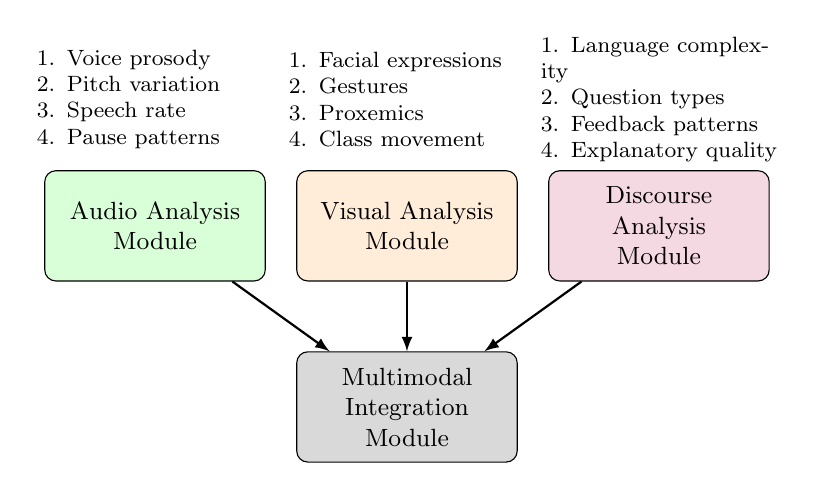
\begin{tikzpicture}[
        module/.style={rectangle, draw, rounded corners, minimum width=2.8cm, minimum height=1.4cm, text width=2.2cm, align=center, font=\small},
        arrow/.style={->, thick, >=latex}
    ]
        % Central component
        \node[module, fill=gray!30] (central) at (0,0) {Multimodal Integration Module};
        
        % Source modules (spaced further apart)
        \node[module, fill=green!15] (audio) at (-3.2,2.3) {Audio Analysis Module};
        \node[module, fill=orange!15] (visual) at (0,2.3) {Visual Analysis Module};
        \node[module, fill=purple!15] (text) at (3.2,2.3) {Discourse Analysis Module};
        
        % Connect modules
        \draw[arrow] (audio) -- (central);
        \draw[arrow] (visual) -- (central);
        \draw[arrow] (text) -- (central);
        
        % Features for each module (moved above and spaced)
        \node[text width=3.0cm, align=left, font=\footnotesize, yshift=0.9cm] at (audio.north) {1. Voice prosody\\2. Pitch variation\\3. Speech rate\\4. Pause patterns};
        \node[text width=3.0cm, align=left, font=\footnotesize, yshift=0.9cm] at (visual.north) {1. Facial expressions\\2. Gestures\\3. Proxemics\\4. Class movement};
        \node[text width=3.0cm, align=left, font=\footnotesize, yshift=0.9cm] at (text.north) {1. Language complexity\\2. Question types\\3. Feedback patterns\\4. Explanatory quality};
    \end{tikzpicture}
    \centering
    \caption{\centering Multimodal system components and feature extraction modules.}
    \label{fig:multimodal_components}
\end{figure}

\begin{enumerate}
    \item \textbf{Audio Module:} Captures speech dynamics using directional microphones positioned strategically in the classroom. The system extracts features related to vocal variety, speech clarity, and emotional tone.
    
    \item \textbf{Visual Module:} Employs two wide-angle cameras (front and rear) to capture teacher movements, gestures, and interactions with students. A deep learning-based pose estimation algorithm tracks key behavioral indicators.
    
    \item \textbf{Discourse Module:} Applies NLP techniques to analyze transcribed classroom dialogue, identifying patterns of instruction, questioning techniques, and feedback quality.
\end{enumerate}

Data collection will occur simultaneously for both evaluation methods during the same teaching sessions to ensure valid comparisons.

\subsection{Data Processing and Feature Extraction}

\subsubsection{Audio Data Processing}
Audio data will be processed to extract the following features:
\begin{itemize}
    \item Prosodic features (pitch, intensity, and speech rate)
    \item Voice quality parameters (jitter, shimmer, and harmonic-to-noise ratio)
    \item Temporal features (speaking time, pause duration, and turn-taking patterns)
    \item Emotion indicators (valence and arousal levels)
\end{itemize}

Audio processing will employ the PRAAT acoustic analysis software with custom scripts for feature extraction, followed by normalization to account for individual voice characteristics.

\subsubsection{Visual Data Analysis}
Visual analysis will focus on extracting behavioral indicators using the following pipeline:

\begin{figure}[t]
    \centering
    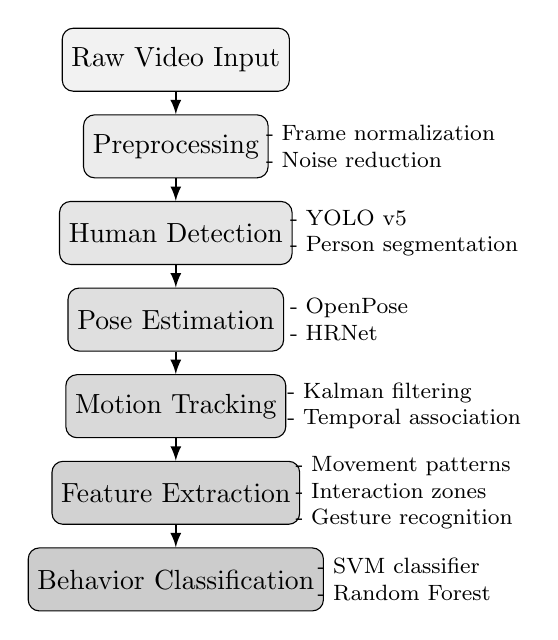
\begin{tikzpicture}[
        stage/.style={rectangle, draw, rounded corners, minimum width=1.8cm, minimum height=0.8cm, align=center, font=\normalsize},
        arrow/.style={->, thick, >=latex}
    ]
        % Processing stages
        \node[stage, fill=gray!10] (input) at (0,0) {Raw Video Input};
        \node[stage, fill=gray!15] (preproc) at (0,-1.1) {Preprocessing};
        \node[stage, fill=gray!20] (detect) at (0,-2.2) {Human Detection};
        \node[stage, fill=gray!25] (pose) at (0,-3.3) {Pose Estimation};
        \node[stage, fill=gray!30] (track) at (0,-4.4) {Motion Tracking};
        \node[stage, fill=gray!35] (extract) at (0,-5.5) {Feature Extraction};
        \node[stage, fill=gray!40] (classify) at (0,-6.6) {Behavior Classification};
        
        % Connect stages
        \draw[arrow] (input) -- (preproc);
        \draw[arrow] (preproc) -- (detect);
        \draw[arrow] (detect) -- (pose);
        \draw[arrow] (pose) -- (track);
        \draw[arrow] (track) -- (extract);
        \draw[arrow] (extract) -- (classify);
        
        % Key techniques
        \node[font=\footnotesize, align=left] at (2.6,-1.1) {- Frame normalization\\- Noise reduction};
        \node[font=\footnotesize, align=left] at (2.9,-2.2) {- YOLO v5\\- Person segmentation};
        \node[font=\footnotesize, align=left] at (2.2,-3.3) {- OpenPose\\- HRNet};
        \node[font=\footnotesize, align=left] at (2.9,-4.4) {- Kalman filtering\\- Temporal association};
        \node[font=\footnotesize, align=left] at (2.9,-5.5) {- Movement patterns\\- Interaction zones\\- Gesture recognition};
        \node[font=\footnotesize, align=left] at (2.9,-6.6) {- SVM classifier\\- Random Forest};
    \end{tikzpicture}
    \caption{ Visual data processing pipeline for teacher behavior analysis.}
    \label{fig:vision_pipeline}
\end{figure}

The system will quantify spatial classroom dynamics, including:
\begin{itemize}
    \item Classroom coverage (percentage of classroom space utilized)
    \item Proximity patterns (time spent in different classroom zones)
    \item Student interaction frequency (number and distribution of individual engagements)
    \item Gesture frequency and type (emphatic, illustrative, and regulatory)
\end{itemize}

\subsubsection{Linguistic and Discourse Analysis}
Classroom dialogue will be transcribed automatically using speech-to-text technology and analyzed for:
\begin{itemize}
    \item Question complexity (based on Bloom's taxonomy)
    \item Wait time after questions
    \item Feedback patterns (evaluative, corrective, or elaborative)
    \item Language complexity (lexical diversity and sentence structure)
    \item Instructional clarity indicators (use of examples, analogies, and summaries)
\end{itemize}

\subsubsection{Student Feedback Processing}
Quantitative feedback will be analyzed using descriptive and inferential statistics, while qualitative comments will undergo thematic analysis using a dual-coding approach to identify emergent patterns. NLP techniques will also be applied to extract sentiment and topical focus from written comments.

\subsection{Evaluation Metrics}
The comparative analysis will employ the following metrics to assess the relationship between traditional and multimodal evaluations:

\begin{table}[t]
    \centering
    \normalsize
    \caption{Evaluation Dimensions and Corresponding Metrics}
    \label{tab:metrics}
    \begin{tabular}{lcc}
        \toprule
        \textbf{Dimension} & \textbf{Student Feedback Metric} & \textbf{Multimodal Metric} \\
        \midrule
        Engagement & Likert rating (1-5) & Interaction frequency + \\
         & & Voice animation index \\
        \midrule
        Clarity & Likert rating (1-5) & Speech rate + Pause ratio + \\
         & & Example frequency \\
        \midrule
        Organization & Likert rating (1-5) & Topic coherence score + \\
         & & Transition clarity index \\
        \midrule
        Responsiveness & Likert rating (1-5) & Response time + \\
         & & Student engagement rate \\
        \bottomrule
    \end{tabular}
\end{table}

Statistical analyses will include:
\begin{itemize}
    \item Correlation analysis between student ratings and multimodal metrics
    \item Factor analysis to identify underlying constructs across evaluation methods
    \item Multiple regression to predict student satisfaction from multimodal features
    \item Paired comparisons to identify systematic differences between methods
\end{itemize}

\subsection{Ethical Considerations}
This research has received approval from the Institutional Review Board (IRB) and implements the following ethical safeguards:
\begin{itemize}
    \item Informed consent from all participating instructors and students
    \item Data anonymization protocols for both traditional and multimodal datasets
    \item Secure data storage with encryption and access controls
    \item Options for participants to review their data and withdraw at any time
    \item Transparent communication about data usage and research findings
\end{itemize}

All classroom recordings will be processed on secure, local servers rather than cloud-based solutions to enhance privacy protection. Face-blurring technology will be applied to student images in accordance with privacy regulations.

% This is now Chapter 4
This section describes the environment, tools, and procedures used to conduct the comparative study between the multimodal teacher evaluation system and traditional student feedback.

\subsection{Classroom Environment}
Experiments were conducted in real university classrooms across three academic departments (STEM, Humanities, Social Sciences). Each classroom was equipped with standard teaching facilities and additional sensors for multimodal data collection.

\subsection{Hardware and Software}
\begin{itemize}
    \item \textbf{Audio:} Directional microphones (Shure MX391) placed at the front and rear of the classroom.
    \item \textbf{Video:} Two wide-angle HD cameras (Logitech C920) positioned to capture both teacher and student interactions.
    \item \textbf{Computing:} A dedicated workstation (Intel i7, 32GB RAM, NVIDIA RTX 3060) for real-time data processing and storage.
    \item \textbf{Software:} 
        \begin{itemize}
            \item PRAAT for audio feature extraction
            \item OpenPose/HRNet for pose estimation
            \item Python (NumPy, pandas, scikit-learn) for data analysis
            \item Custom NLP pipeline for discourse analysis
        \end{itemize}
\end{itemize}

\begin{table}[H]
    \centering
    \normalsize
    \caption{Summary of Collected Dataset}
    \label{tab:dataset_summary}
    \begin{tabular}{lcc}
        \toprule
        \textbf{Data Type} & \textbf{Sessions} & \textbf{Total Size} \\
        \midrule
        Audio & 90 & 18 hours (12 GB) \\
        Video & 90 & 18 hours (90 GB) \\
        Transcripts & 90 & 1.2M words (8 MB) \\
        Student Feedback & 90 & 1,350 responses (0.5 MB) \\
        \bottomrule
    \end{tabular}
\end{table}


\subsection{Data Collection Procedure}
\begin{enumerate}
    \item \textbf{Session Preparation:} Instructors and students were briefed and consent was obtained. Equipment was set up before each session.
    \item \textbf{Recording:} Each teaching session (50 minutes) was recorded for both audio and video. Student feedback was collected immediately after each session via online forms.
    \item \textbf{Synchronization:} All data streams were time-synchronized using a central clock to ensure accurate multimodal analysis.
    \item \textbf{Data Storage:} Raw data was securely stored on encrypted local drives. Only anonymized data was used for analysis.
\end{enumerate}

\subsection{Dataset Overview}
A total of 90 teaching sessions were recorded (30 instructors × 3 sessions each). For each session, the following data was collected:
\begin{itemize}
    \item Audio recordings (WAV, 44.1kHz)
    \item Video recordings (MP4, 1080p)
    \item Automatic transcripts (TXT)
    \item Student feedback responses (CSV)
\end{itemize}


% This is now Chapter 5

The proposed system is a modular, end-to-end multimodal machine learning pipeline that processes audio, video, and transcript data streams in parallel, fuses their representations, and predicts teaching effectiveness using a unified classifier. This architecture leverages state-of-the-art models and best practices from the HuggingFace ecosystem and the broader machine learning community.

\begin{figure}[H]
    \centering
    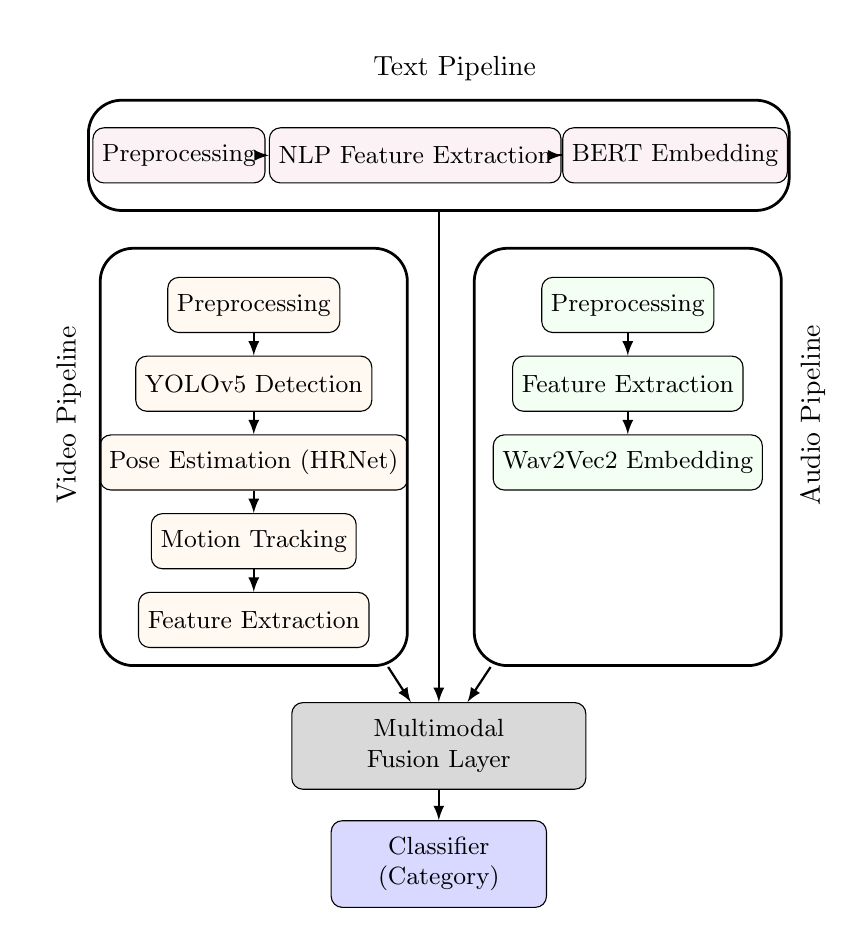
\begin{tikzpicture}[
        module/.style={rectangle, draw, rounded corners, minimum width=2.5cm, minimum height=1.1cm, text width=2.5cm, align=center, font=\small, fill=gray!10},
        arrow/.style={->, thick, >=latex},
        process/.style={rectangle, draw, rounded corners, minimum width=2cm, minimum height=0.7cm, font=\small, fill=white},
        pipelinebox/.style={draw=black, rounded corners=12pt, line width=1pt, minimum width=3.2cm, minimum height=5.3cm}
    ]

        % Text pipeline
        \node[process, fill=purple!5] (t1) at (-6.2,3.3) {Preprocessing};
        \node[process, fill=purple!5] (t2) at (-3.2,3.3) {NLP Feature Extraction};
        \node[process, fill=purple!5] (t3) at (0.1,3.3) {BERT Embedding};
        \node[pipelinebox,rotate=0, minimum width=8.9cm,minimum height=1.4cm, fill=none] (cover3) at (-2.9,3.3) {};
        \node[label, rotate=0, xshift=-2.7cm,yshift=4.4cm] {Text Pipeline};

        % Video pipeline
        \node[process, fill=orange!5] (v1) at (-5.25,1.4) {Preprocessing};
        \node[process, fill=orange!5] (v2) at (-5.25,0.4) {YOLOv5 Detection};
        \node[process, fill=orange!5] (v3) at (-5.25,-0.6) {Pose Estimation (HRNet)};
        \node[process, fill=orange!5] (v4) at (-5.25,-1.6) {Motion Tracking};
        \node[process, fill=orange!5] (v5) at (-5.25,-2.6) {Feature Extraction};
        \node[pipelinebox,minimum width=3.9cm, fill=none] (cover1) at (-5.25,-.53) {};
        \node[label, rotate=90, xshift=0cm,yshift=7.6cm] {Video Pipeline};


        % Audio pipeline
        \node[process, fill=green!5] (a1) at (-0.5,1.4) {Preprocessing};
        \node[process, fill=green!5] (a2) at (-0.5,0.4) {Feature Extraction};
        \node[process, fill=green!5] (a3) at (-0.5,-0.6) {Wav2Vec2 Embedding};
        \node[pipelinebox, minimum width=3.9cm,fill=none] (cover2) at (-0.5,-.53) {};
        \node[label, rotate=90, xshift=0cm,yshift=-1.85cm] {Audio Pipeline};

       

        % Fusion and classifier
        \node[module, fill=gray!30, minimum width=3.5cm, text width=3.5cm] (fusion) at (-2.9,-4.2) {Multimodal Fusion Layer};
        \node[module, fill=blue!15, minimum width=2.5cm, text width=2.5cm] (clf) at (-2.9,-5.7) {Classifier\\(Category)};

        % Arrows for video
        \draw[arrow] (v1) -- (v2);
        \draw[arrow] (v2) -- (v3);
        \draw[arrow] (v3) -- (v4);
        \draw[arrow] (v4) -- (v5);
        \draw[arrow] (cover1) -- (fusion);

        % Arrows for audio
        \draw[arrow] (a1) -- (a2);
        \draw[arrow] (a2) -- (a3);
        \draw[arrow] (cover2) -- (fusion);

        % Arrows for text
        \draw[arrow] (t1) -- (t2);
        \draw[arrow] (t2) -- (t3);
        \draw[arrow] (cover3) -- (fusion);

        % Fusion to classifier
        \draw[arrow] (fusion) -- (clf);

    \end{tikzpicture}
    \centering
    \caption{High-level architecture of the proposed multimodal teacher evaluation system. Each modality is processed by a dedicated pipeline; their features are fused with session metadata and classified.}
    \label{fig:multimodal_architecture}
\end{figure}

\subsection{Video Stream pipeline}  
\begin{itemize}
    \item \textbf{Preprocessing:} Video frames are normalized and denoised.
    \item \textbf{Human Detection:} YOLOv5 (via HuggingFace) detects all people in each frame.
    \item \textbf{Pose Estimation:} HRNet or OpenPose extracts skeletal keypoints for each detected person.
    \item \textbf{Motion Tracking:} Kalman filtering links poses across frames to track teacher movement.
    \item \textbf{Feature Extraction:} Computes gesture frequency, classroom coverage, interaction zones, and movement patterns \cite{mcneill1992hand}.
\end{itemize}

\subsection{Audio Stream pipeline}  
\begin{itemize}
    \item \textbf{Preprocessing:} Audio is denoised and segmented.
    \item \textbf{Feature Extraction:} PRAAT and Python extract prosodic features (pitch, intensity, speech rate) and emotion embeddings.
    \item \textbf{Audio Embedding:} Wav2Vec2 (HuggingFace Transformers) produces deep audio representations.
\end{itemize}

\subsection{Text Stream pipeline}  
\begin{itemize}
    \item \textbf{Preprocessing:} Transcripts are cleaned and tokenized.
    \item \textbf{NLP Feature Extraction:} Sentiment analysis, question type detection, and discourse structure are computed \cite{sinclair1975discourse}.
    \item \textbf{Text Embedding:} BERT or DistilBERT (HuggingFace Transformers) generates semantic embeddings.
\end{itemize}

\subsection{Multimodal Fusion and Classification}  
\begin{itemize}
    \item \textbf{Fusion Layer:} All modality embeddings/features are concatenated and combined with session metadata (e.g., class size, subject).
    \item \textbf{Classifier:} The fused vector is input to a fully connected neural network with a softmax (for categorical) or regression (for continuous) output, predicting teaching effectiveness.
\end{itemize}

\textbf{Modeling and Training:}  
\begin{itemize}
    \item All models are implemented in PyTorch, leveraging HuggingFace Transformers for pretrained components.
    \item Training follows standard ML protocols: stratified train/validation/test splits, cross-entropy or MSE loss, Adam optimizer, and early stopping.
    \item Cross-modal alignment is ensured by synchronizing timestamps and using late fusion for interpretability.
    \item The system is modular and extensible, allowing new modalities or metadata to be added with minimal changes.
\end{itemize}

\textbf{Privacy and Ethics:}  
All data is anonymized; student faces are blurred in video, and all processing is performed on secure, local servers.

This detailed implementation ensures the system is robust, interpretable, and aligned with current machine learning standards for multimodal educational analytics.

\subsection{System Output and Classification}

The output of our multimodal teacher evaluation system is a categorical label that summarizes the overall teaching effectiveness for each observed session. This label is generated by the classifier based on fused features from audio, video, and transcript data, as well as session metadata. The categories are designed to be both interpretable and actionable, providing clear feedback to educators and administrators without excessive granularity or oversimplification.

The classification is as follows (see Table~\ref{tab:output_categories}):

\begin{table}[t]
    \centering
    \normalsize
    \caption{Teacher Evaluation Output Categories}
    \label{tab:output_categories}
    \begin{tabular}{p{2.2cm} p{7.1cm}}
        \toprule
        \textbf{Category} & \textbf{Description} \\
        \midrule
        Outstanding & Consistently exceeds expectations in all evaluation dimensions. \\
        Very Good & Frequently exceeds expectations; minor areas for growth. \\
        Good & Meets expectations in most areas; some strengths and some areas to improve. \\
        Satisfactory & Adequate performance; meets minimum standards but with clear room for improvement. \\
        Needs Improvement & Below expectations in several areas; targeted development required. \\
        Unsatisfactory & Consistently below standards; significant intervention needed. \\
        \bottomrule
    \end{tabular}
\end{table}

Each session is assigned one of these categories, which can be used for formative feedback, professional development planning, or institutional reporting. The system is also capable of providing a confidence score for each prediction, and can generate a brief textual summary highlighting the key factors influencing the classification (e.g., engagement level, clarity, responsiveness). This approach ensures that the output is both meaningful and actionable for stakeholders.

\begin{table*}[htbp]
\centering
\renewcommand{\arraystretch}{1.5} % Increase row padding
\setlength{\tabcolsep}{8pt} % Increase column padding
\caption{Pedagogical Dimensions Mapped to Multimodal Features with Supporting Literature}
\begin{tabular}{|p{3cm}|p{4.5cm}|p{4.5cm}|p{3.8cm}|}
\hline
\textbf{\normalsize Dimension} & \textbf{\normalsize Audio Features} & \textbf{\normalsize Visual Features} & \textbf{\normalsize Linguistic Features} \\
\hline

\textbf{Engagement} & 
Pitch variability, speech rate, intensity, arousal level \cite{hou2024encouragement, dmello2012multimodal} & 
Interaction frequency, gesture frequency, classroom coverage \cite{mcneill1992hand, ochoa2016multimodal} & 
None specific \cite{hou2024encouragement, dmello2012multimodal} \\ 
\hline

\textbf{Clarity} & 
Speech rate, pause ratio, vocal jitter/stability \cite{falcon2024discourse, rowe1986wait} & 
Frontal stance, head pose (gaze alignment), low distraction movement \cite{mcneill1992hand, ochoa2016multimodal} & 
Sentence structure, use of examples, summaries, lexical clarity \cite{falcon2024discourse, rowe1986wait} \\
\hline

\textbf{Organization} & 
Turn-taking structure, speaking time distribution \cite{ochoa2016multimodal, dmello2012multimodal} & 
Movement between zones (topic transitions), spatial consistency \cite{mcneill1992hand, ochoa2016multimodal} & 
Discourse coherence, topic structure, transitions \cite{ochoa2016multimodal, dmello2012multimodal} \\
\hline

\textbf{Responsiveness} & 
Response latency, dynamic pitch, prosodic emphasis \cite{rowe1986wait, dmello2012multimodal} & 
Proximity to students when responding, frequency of engagement moments \cite{mcneill1992hand, ochoa2016multimodal} & 
Feedback types (evaluative, corrective, elaborative), wait time \cite{rowe1986wait} \\
\hline

\textbf{Emotional Climate} & 
Valence and arousal scores from emotional prosody \cite{dmello2012multimodal} & 
Facial expressions, expressive gestures \cite{mcneill1992hand, ochoa2016multimodal} & 
Sentiment polarity, affective markers \cite{dmello2012multimodal} \\
\hline

\textbf{Inclusivity \& Accessibility} & 
Turn balance (teacher vs. students), speaking time equity & 
Gaze distribution, equal visual attention, gesture openness \cite{fugate2010gaze} & 
Lexical simplicity, inclusive language, diverse addressing styles \cite{Steinberg2021, Heffernan2022} \\
\hline

\textbf{Cognitive Activation} & 
Pitch intensity shifts for emphasis & 
Dynamic posture during questioning & 
Bloom's Taxonomy question complexity levels \cite{graesser2005question, chi1989self} \\
\hline

\end{tabular}
\end{table*}



\section{Results and Discussion}
Present the findings of the comparative study here. Include quantitative and qualitative results, statistical analyses, and a discussion interpreting the significance of the results in the context of existing literature.

\section{Conclusion and Future Work}
Summarize the main contributions and findings of the study. Discuss limitations and propose directions for future research.

\section*{Acknowledgment}
(Optional) Acknowledge any funding sources, institutional support, or individuals who contributed to the research but are not listed as authors.

\bibliographystyle{IEEEtran}
\bibliography{research}

\end{document}